\documentclass[crop,tikz]{standalone} 
\usepackage{tikz, amsmath, amssymb, graphicx} 

\DeclareMathAlphabet\mathbfcal{OMS}{cmsy}{b}{n}

\newcommand{\Mt}{\mathbfcal{M}}
\newcommand{\Yt}{\mathbfcal{Y}}
\newcommand{\Ft}{\mathbfcal{F}}

\usetikzlibrary{positioning, shapes.geometric} 

\begin{document} 

\begin{tikzpicture}


\node[inner sep=0pt] (sim:0.05) at (0,0) {
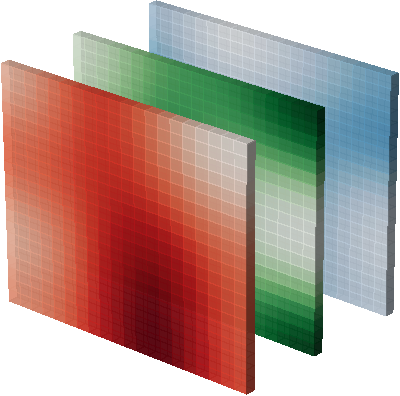
\includegraphics[width=0.3\textwidth]{F.pdf}
};

\node[inner sep=0pt] (sim:0.05) at (4.5,0) {
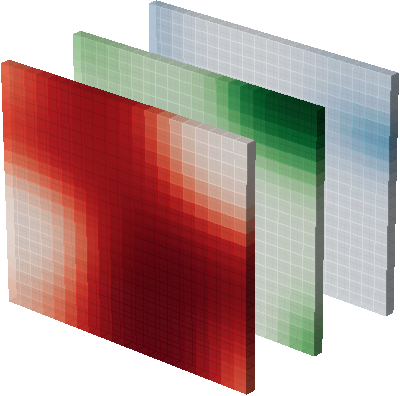
\includegraphics[width=0.3\textwidth]{Mu.pdf}
};


\node[inner sep=0pt] (sim:0.05) at (9,0.1) {

\includegraphics[width=0.25\textwidth]{Y.pdf}
};



\draw (0, 2.3) node {$\Ft$};
\draw (4.5,2.3) node {$\Mt$};
\draw (9,2.3) node {Most likely classification};




% \draw (6.8,2.7) node {CGM};

% \draw (-4.2,0.3) node {$m=0.05$};
% \draw (-4.2,-4.7) node {$m=0.5$};
% \draw (-4.2,-9.7) node {$m=0.95$};


\end{tikzpicture}
\end{document} 
